\chapter{Project Methodology}
In this chapter we will describe the project methodology that we have applied to this project.
We will first talk about a global planning for the project.
Here we will divide the project into three phases.
After this we will talk about an overall process strategy and what strategy we will apply to which phase and why.
Thirdly, we will talk about which team member has which project roles and what these project roles imply.
After this we will talk about each of the three phases in more detail about their individual planning and deliverables.
Here we will also reflect on the phase and talk about what went wrong and what went right.
Lastly, we define the tools that we have used during the project.

\section{Global planning}
In figure~\ref{global_planning} you can see the global planning that we have set up.
It mentions all the big deliverables and gives the team a good overview of how far the progress of the project should be.
The team can compare the current state of the project with this planning and can conclude if there is sufficient progress and if measures should be undertaken.

\begin{figure}[h]
    \centering
    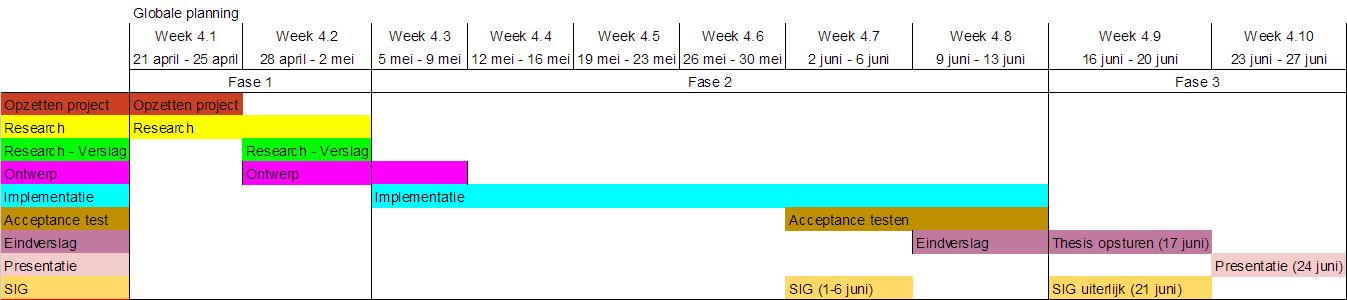
\includegraphics[width=\textwidth]{images/Global_planning}
    \caption{Global planning of the project}
    \label{global_planning}
\end{figure}

As you can see in the image, we divided the project into three phases:
\begin{itemize}
\item Research and set-up (phase 1)
\item Design and implementation (phase 2)
\item Testing, documentation and presentation (phase 3)
\end{itemize}
Each of these phases describes the things that need to be done during that phase.
Not all tasks are completely in one phase, they overlap between two phases.
To know how far we have progressed, we specified a week where the task should start and when it should end.
In the sections about the phases we will go into further detail about the deliverables and planning of each phase.

\section{Overall process strategy}
We started the project off without a strict task distribution.
We choose to do so because many of the tasks at hand needed group thinking and group opinions.
For example, the interpretation of the problem description is something that can be thought out by a single person, but needs to be communicated to and discussed with the other team members.
If not communicated enough, the resulting problem description may not be the same as how the team interpreted the client's description.\\
The tasks that needed to be done were documented in a spreadsheet.
In this way, every team member had insight into the things that still needed to be done.
Each team member could claim a task for himself when he finished his last task.
That way a quick look into the spreadsheet will give you a good overview of which tasks were important within a short time notice.

\subsection{Meetings}
Although the team spends most of the week together working on the project, it is still necessary to plan weekly meetings.
These meetings help with spending time dedicated with talking through the current progress of the project and possible problems that we could encounter.
The meetings are planned at the beginning of each week, so that we could discuss what has been done last week and what needs to be done the upcoming week.
It also helps identifying the things that need to be done. These things were added to the spreadsheet after the meeting.

\subsection{Software development method}\label{software_development_method}
During the implementation phase we used a known software development framework.
This development framework is known as scrum.
Scrum is based on the agile software development framework which can be used to 
manage software projects.
The time that we have to implement the system is limited so we did not have the time to research and design all aspects of the system. We need a software development framework that gave us the possibility to react to changes in requirements, but also to react to new insights given by our increasing understanding of the system as time progresses.
Scrum has a flexible approach to software development and satisfies the requirements that we have mentioned above.
In scrum, you only need a basic design of the system before you start implementing.
During implementation you provide daily feedback on your progress and the team can change the way things are programmed or have been programmed to steer the product in the proper direction.
During the research into scrum we ran into the problem that scrum required us to divide roles between team members (e.g. the product owner, development team, scrum master).
We choose to also divide the bigger remaining responsibilities among the team members.
In this way we could ensure that each team member had his own responsibilities and that no aspect of the project would fall behind.
In the next section we define the different roles and divide them among the team members.

\section{Project roles}
As said above, in the beginning there was not a strict task distribution.
Following the advise of our group mentor, every week a different team member was the designated chairman and another team member was the designated secretary.
The chairman of the week had the responsibility to preside the weekly meetings and to maintain an overview of the tasks that were at hand.
The secretary had the responsibility of making minutes of both the weekly meetings and the meetings with the group mentors and client.
These two roles stayed the same throughout the project.

As said above, we realised that we needed more defined roles.
We defined the following roles:
\begin{itemize}
\item Lead Development, is responsible for the implementation phase;
\item Scrum master, is responsible for the scrum process;
\item Quality Assurance, is responsible for the quality of code and test coverage;
\item Project Manager, is responsible for maintaining an overview of the project and making sure the product is finished on time;
\item Lead Documentation, is responsible for the documentation of the various aspects of the project.
\end{itemize}

The following table lists the different group members and their roles.\\
\begin{tabular}{|l|l|}
\hline
Name & Roles\\
\hline
Freek van Tienen & Lead Development\\
\hline
Floris Verburg & Scrum master and Quality Assurance\\
\hline
Marijn Goedegebure & Project Manager and Reports\\
\hline
\end{tabular}

\section{Phase 1}
\subsection{Goal}
The first phase aims to expand the knowledge of the group about the problem and it's requirements.
Secondly, it also gives time for the team members to analyse the problem for difficult subjects and to spend time finding a fitting solution.
Thirdly it gives the team members the time to set up the project infrastructure and to define the project methodology.
Lastly, the remaining time should be spend making a first start with the system design.

\subsection{Planning}
We planned phase 1 to be two weeks long.
With the first week having a focus on setting up the project and doing research to the problem and requirements.
The second week was more about defining the project methodology, analysing and researching the possible problems that we could encounter and making a first system design.
The second week was also used to finish up the research report.

\subsubsection{Planned deliverables}
At the end of phase 1 we wanted to have the following deliverables done:
\begin{itemize}
\item Research report
\item Plan of approach
\item First system design
\end{itemize}

\subsection{Process strategy}
During this phase we choose to not have a strict task distribution.
Many of the tasks at hand needed group thinking and group opinions.
For example, the interpretation of the problem description is something that can be thought out by a single person, but needs to be communicated about toward the other team members.
If not communicated enough, the resulting problem description may not be the same as how the team interpreted the client's description.
Things that needed to be done were documented in a spreadsheet.
In this way, every team member had insight into the things that still needed to be done.

\subsection{Phase reflection}
During the first phase we had some trouble with determining the direction that the project would take.
Although the Computer Science bachelor has a lot of projects, this is the first project that you are completely free.
This gave us some problems at the start of the project.
After reading up on some projects that were done last few years, we had a better insight into what was expected from us.
During the first week we made good progress with defining the requirements, but later realised that we probably should have started with the plan of approach.
We made sure to catch up in this regard.

We also spend some time during the first week in setting up the programming environment.
Because of this we suffered some delay with the research report.
This wasn't a big problem, because otherwise we would have done it right after the research report and both the research report and the plan of approach didn't have a completion date.
This might even have worked in our favour by giving us time to have another meeting with our supervisors and discussing the direction and progress of the project.
We used the third week of the project to catch up on the research report.

The other delivery was the first system design, this is not a properly defined deliverable but was more an indication that we should have started on this.
We did so by choosing to develop a web application.

Despite the rough start, in retrospect we are happy with the result of the first two weeks.
It gave us a good start for the implementation phase and we didn't have many set backs.

\section{Phase 2}
\subsection{Goal}
The purpose of the second phase was to provide a time frame in which both a basic system design can be made and the system design could be implemented.
During the second phase the roles were more strict since we wanted to follow a structured software development method.
This software development method is the framework known as scrum.
We will go into depth about this in the process strategy section.

\subsection{Planning}
We planned the second phase to be six weeks long.
The first week was used to finish up the system design.
The other 5 weeks were used to implement this system design.
During the final two weeks we looked into the user tests and the acceptance tests.
During this time there we also sent our source code to the Software Improvement Group for them to check.
The feedback that we got back will be discussed later in this paper.

\subsubsection{Planned deliverables}
During phase two we wanted to have the following deliverables done:
\begin{itemize}
\item Basic system design
\item User tests
\item Send the source code to SIG for the first review
\item A working application
\end{itemize}

\subsection{Phase reflection}
During this phase the main task of the team was implementing the system design.
The first task of the team was to complete the system design.
This needed a couple team meetings discussing the database design and the interface interaction.
After completing this, the implementation could start.
Not many problems were encountered during the implementation.
During the implementation we didn't always did a pull request per feature.
Some features were just to big to do this.
This was caused by not having a lot of experience with such big projects and the possibility that features can be so big.
We resolved this by splitting up the pull request in multiple parts.

We also thought the reviewing of the pull requests to be very useful.
This helps to have all the team members be up to date with the newest features added to the system.

It also helped checking the code for human errors.
During this phase we used our continuous integration solution to analyse our code and to run automated tests on the system.
We thought the static analysis to be very useful, it increases the readability of the code a lot.
The automated tests also helped, by decreasing the checking needed by the team members.

We are very happy how the implementation phase went.
The amount of features that we implemented did not stall anywhere during the process.
We wonder if we made the right choice by spending a moderate amount of time improving our interface.
It belongs to the making of a complete product, but it also means that we did not have the chance to implement more features.

\section{Phase 3}
\subsection{Goal}
The goal of the third and last phase is to provide for time to finish up the project.
During this phase time has been reserved for finishing up the implementation, the final report and for the user tests.

\subsection{Planning}
During this phase there is time for completion of the implementation, finalisation of the final report and creation of the presentation.
The completion of the implementation and the finalisation of the final report will been done simultaneously.
The creation of the presentation will be done after the final report has been submitted.
After the final report is submitted we will also be looking into the feedback that we received from the SIG.
Three days before the presentation, the source code should be send to SIG for a final review.

\subsubsection{Planned deliverables}
During phase three we wanted to have the following deliverables done:
\begin{itemize}
\item Final report
\item Presentation
\item Improved implementation following the comments provided by SIG
\item Final review of SIG
\end{itemize}

\subsection{Phase reflection}
During the final phase the goal was to finish up the project.
The main tasks were the user tests, integration tests and the final report.
The planning for the last phase was strict, we did not have much manoeuvrability or time to delay.
First up was the final report which you are reading now.
We needed to work through the weekend to finish it up in time, but it was mostly to make sure that we weren't stressing too much.
That also gave us the possibility to send our report to our supervisors for a review before the final draft.

At the end of the second phase we sent our source code to SIG for checking.
Later in this paper we will discuss the comments that SIG made.
During the final presentation we will comment on the final review that SIG has made.

While the final report will soon be done, the final presentation and final review will not be complete until after the report has been completed.
We have a week from the deadline of the final report until our presentation.
In this time the following things need to be done:
\begin{itemize}
\item Create the presentation
\item Improve implementation using the feedback of SIG
\item Prepare the live demo for the presentation
\end{itemize}
We think that the remaining week until the presentation will be enough time for these deliverables.

\section{Tools}
We have used several tools to support our project.
The tools helped in administrative work, but also in improving code quality and maintainability.
In the following list we mention each tool that we used and the benefit that it has.

\begin{itemize}
\item IntelliJ IDEA, is our Integrated Development Environment (IDE) which will facilitate the development and testing of our code.
IntelliJ will be integrated with the Play framework which will be helpful during development.
\item GitHub, is our on-line code and documentation repository.
It provides for a version control system, an issue tracker and code review possibilities.
We will be using it to store all our code and documentation's code (LaTeX).
\item Cloudbees
Cloudbees will be used to run our test environment, our continuous integration and the release environment.
It uses Jenkins for the continuous integration.
\item Play framework
The play framework gives us the possibility to easily create a web application using Java.
\item Findbugs is a plug in for Cloudbees and IntelliJ that gives us the possibility to let our java code be checked for small bugs using static analysis.
\item JaCoCo is a plug in for Cloudbees and IntelliJ that provides us with data analysis about our code coverage.
\item Checkstyle is a plug in for Cloudbees and IntelliJ that checks the code for coding standards.
This makes it ideal to enforce the coding standard for our project.
\end{itemize}
